% Dodelat odkazy a obrazky

\subsubsection{Description}
%Describe your concept of the RTDS, how the sound is produced, what are the parameters for activating the RTDS, etc.

We use piezo siren AE20M. The siren makes sound when ECUB recognize ready-to-drive state of car, it receives message from ECUF about TS ON button and SDC is in non-error state, if message would be lost ECUB doesn’t send confirmation status and ECUF does not allow to activate ready to drive status. Sound pressure level of this siren is more than 90 dB(A) at 1 m, Output frequency is from 2,9 kHz. Controlling of RTDS is done by ECUB by transistor. RTDS beeps 2 seconds.

\begin{figure}[H]
	\centering
	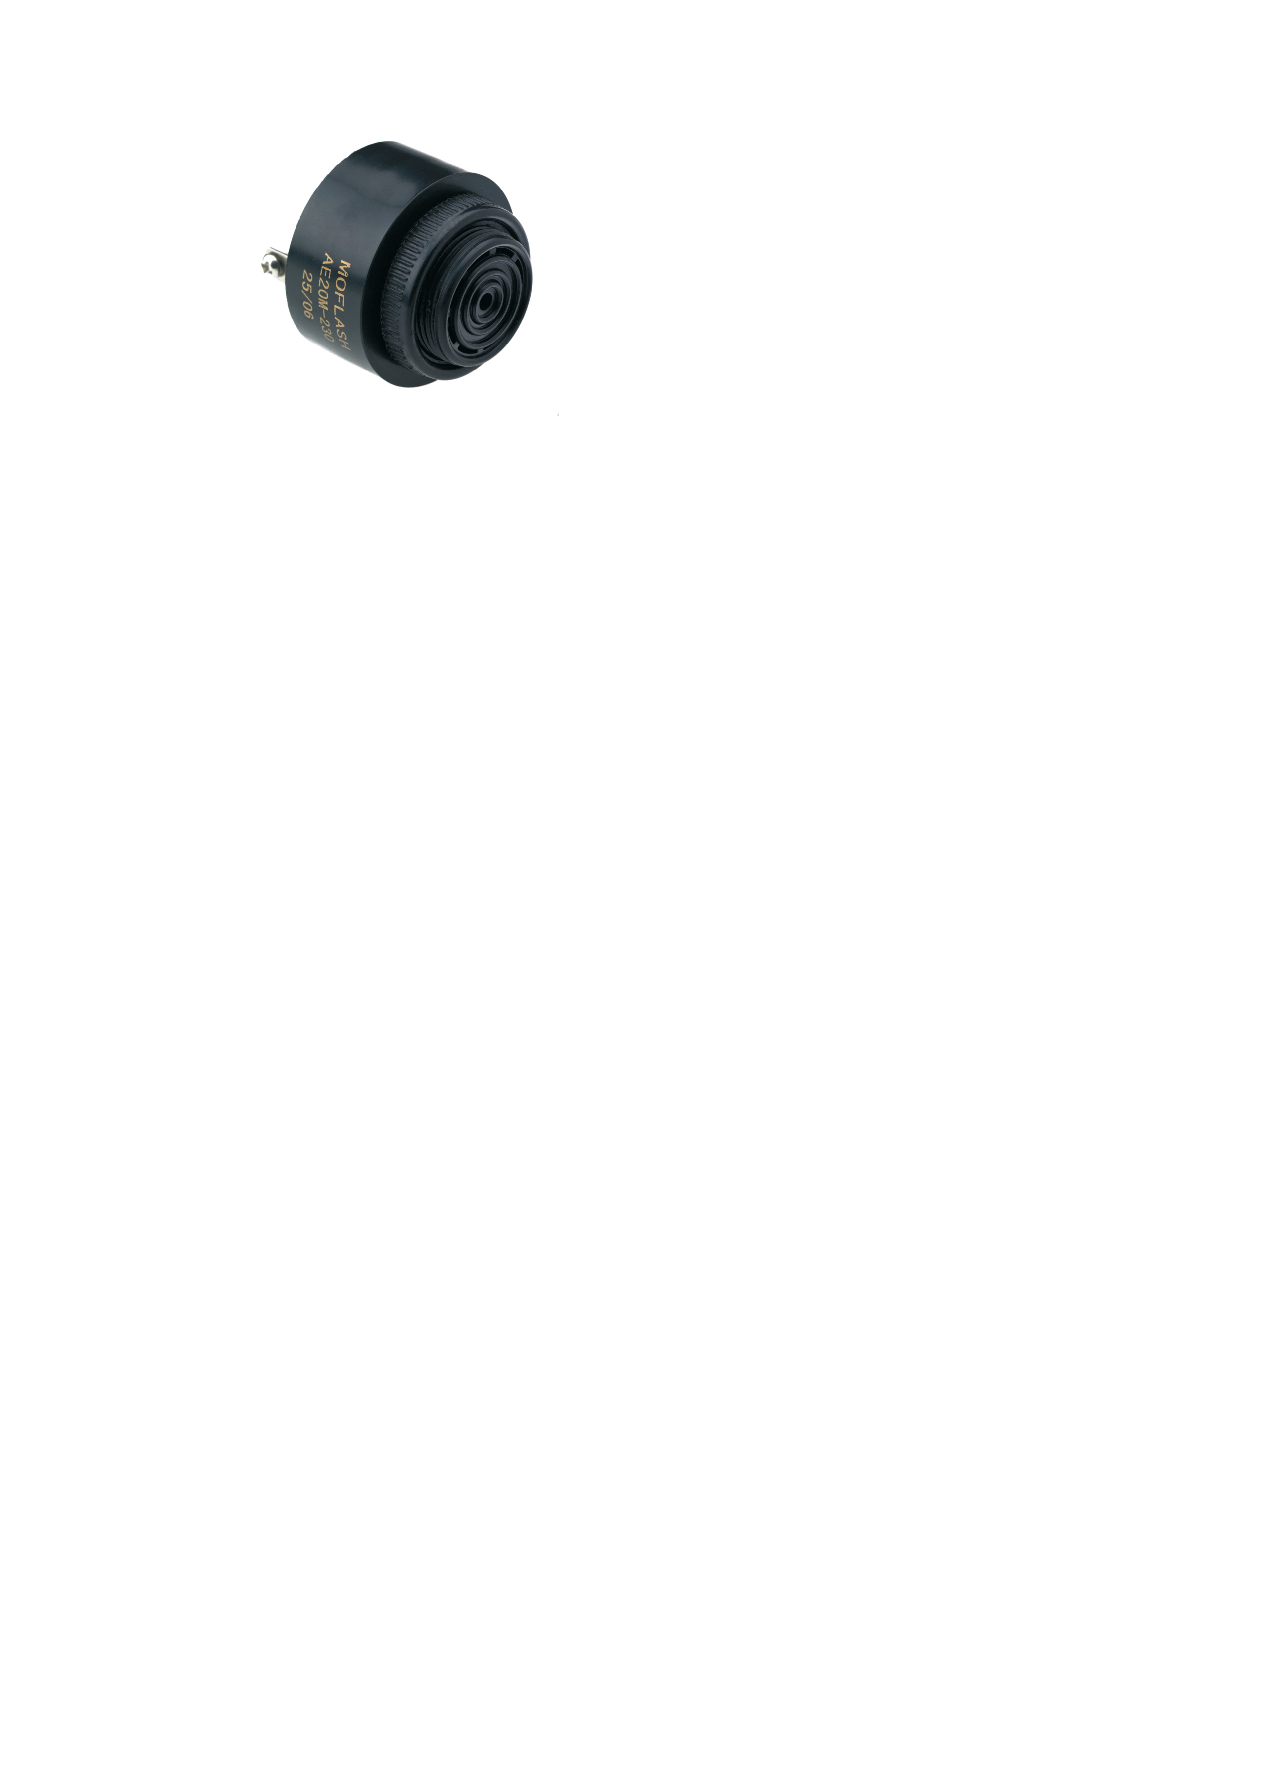
\includegraphics[width=.5\textwidth]{./img/RTDS.pdf}
	\caption{RTDS.}
	\label{fig:RTDS}
\end{figure}

\subsubsection{Wiring, cables, current calculations, connectors}
%Describe wiring, show schematics, describe connectors and cables and show useful data regarding the wiring.

There are only two wires from ECUB to RTDS piezo siren, one switched by transistor and and the second is ground (block connections is on \ref{fig:RTDS-wiring}).

\begin{figure}[H]
	\centering
	
\includegraphics[width=\textwidth]{./img/rtds-wiring.jpg}
	\caption{RTDS wiring.}
	\label{fig:RTDS-wiring}
\end{figure}
\subsubsection{Position in car}
%Provide CAD-renderings showing all relevant parts. Mark the parts in the rendering, if necessary.

Ready to drive sound is placed on the top of Accumulator Pack next to the Motor Controller, see \ref{fig:RTDS-position}.
\begin{figure}[H]
	\centering
	
\includegraphics[width=\textwidth]{./img/rtds-position.jpg}
	\caption{RTDS position.}
	\label{fig:RTDS-position}
\end{figure}